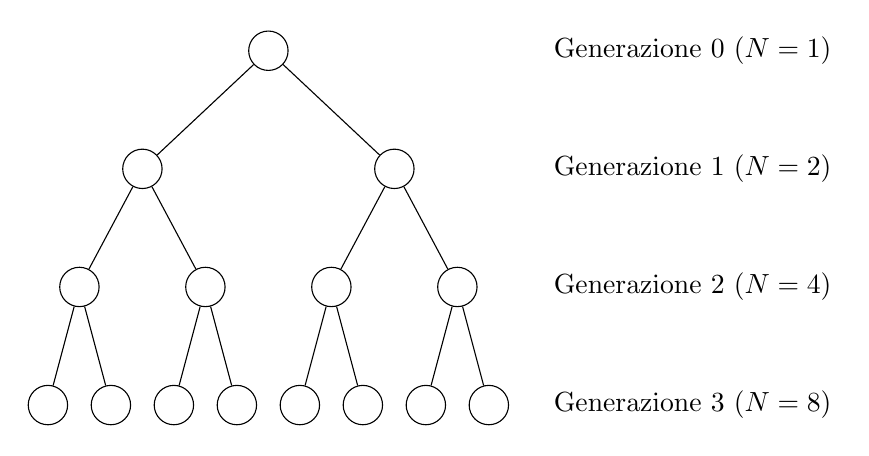
\begin{tikzpicture}[node distance=15mm, main node/.style={circle,draw,minimum size=5mm}]%
  \node at (0, 0) {};
  \node[main node] (1) {};
  \node (l1)[right of=1,xshift=2cm,anchor=west] {Generazione 0 ($N=1$)};
  
  \node[main node] (11) [below of=1, xshift=-16mm] {};
  \node[main node] (12) [below of=1, xshift=16mm] {};
  \draw[] (1) -- (11);
  \draw[] (1) -- (12);
  \node (l2) [below of=l1] {Generazione 1 ($N=2$)};

  \node[main node] (111) [below of=11, xshift=-8mm] {};
  \node[main node] (112) [below of=11, xshift=8mm] {};
  \node[main node] (121) [below of=12, xshift=-8mm] {};
  \node[main node] (122) [below of=12, xshift=8mm] {};
  \draw[] (11) -- (111);
  \draw[] (11) -- (112);
  \draw[] (12) -- (121);
  \draw[] (12) -- (122);
  \node (l3) [below of=l2] {Generazione 2 ($N=4$)};

  \node[main node] (1111) [below of=111, xshift=-4mm] {};
  \node[main node] (1112) [below of=111, xshift=4mm] {};
  \node[main node] (1121) [below of=112, xshift=-4mm] {};
  \node[main node] (1122) [below of=112, xshift=4mm] {};
  \node[main node] (1211) [below of=121, xshift=-4mm] {};
  \node[main node] (1212) [below of=121, xshift=4mm] {};
  \node[main node] (1221) [below of=122, xshift=-4mm] {};
  \node[main node] (1222) [below of=122, xshift=4mm] {};
  \draw[] (111) -- (1111);
  \draw[] (111) -- (1112);
  \draw[] (112) -- (1121);
  \draw[] (112) -- (1122);
  \draw[] (121) -- (1211);
  \draw[] (121) -- (1212);
  \draw[] (122) -- (1221);
  \draw[] (122) -- (1222);
  \node (l4) [below of=l3] {Generazione 3 ($N=8$)};
\end{tikzpicture}

